\documentclass[12pt]{article}
\usepackage{amsfonts, amssymb, amsmath, amsthm}
\usepackage[margin=1in]{geometry}
\usepackage{tikz}
\usetikzlibrary{patterns, decorations.pathreplacing}

\pagestyle{myheadings}
\markright{Explainer: Rudin 4.14 --- Fixed Point Theorem\hfill}

\newcommand{\R}{\mathbb{R}}

\begin{document}

\begin{center}
    \textbf{\Large The Fixed Point Theorem on $[0,1]$}\\[0.5em]
    \large A visual guide to Rudin 4.14
\end{center}

\section{What is a Fixed Point?}

A \textbf{fixed point} of $f$ is a value $x$ where $f(x) = x$ --- the function ``fixes'' $x$ in place.

Graphically: where the curve $y = f(x)$ crosses the line $y = x$.

\begin{center}
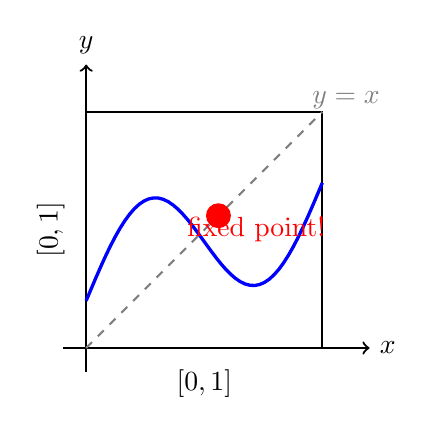
\begin{tikzpicture}[scale=3]
    % Unit square
    \draw[thick] (0, 0) rectangle (1, 1);
    \draw[thick, ->] (-0.1, 0) -- (1.2, 0) node[right] {$x$};
    \draw[thick, ->] (0, -0.1) -- (0, 1.2) node[above] {$y$};

    % y = x line
    \draw[gray, thick, dashed] (0, 0) -- (1, 1);
    \node[gray] at (1.1, 1.05) {$y = x$};

    % A continuous function from I to I
    \draw[blue, very thick, domain=0:1, samples=50] plot (\x, {0.2 + 0.5*\x + 0.3*sin(360*\x)});

    % Fixed point
    \fill[red] (0.56, 0.56) circle (1.5pt);
    \node[red] at (0.72, 0.5) {fixed point!};

    % Labels
    \node at (0.5, -0.15) {$[0, 1]$};
    \node at (-0.15, 0.5) [rotate=90] {$[0, 1]$};
\end{tikzpicture}
\end{center}

\section{The Claim}

\begin{center}
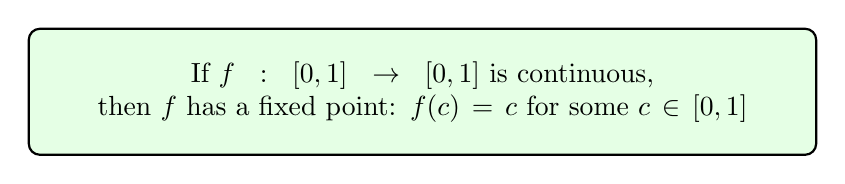
\begin{tikzpicture}
    \draw[thick, rounded corners, fill=green!10] (-5, -0.8) rectangle (5, 0.8);
    \node[text width=9cm, align=center] at (0, 0) {
        If $f: [0,1] \to [0,1]$ is continuous,\\
        then $f$ has a fixed point: $f(c) = c$ for some $c \in [0,1]$
    };
\end{tikzpicture}
\end{center}

\section{Why Must the Curve Cross $y = x$?}

\begin{center}
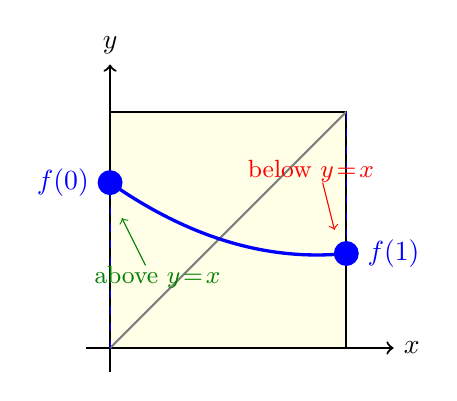
\begin{tikzpicture}[scale=3]
    % Unit square
    \fill[yellow!10] (0, 0) rectangle (1, 1);
    \draw[thick] (0, 0) rectangle (1, 1);
    \draw[thick, ->] (-0.1, 0) -- (1.2, 0) node[right] {$x$};
    \draw[thick, ->] (0, -0.1) -- (0, 1.2) node[above] {$y$};

    % y = x line
    \draw[gray, thick] (0, 0) -- (1, 1);

    % Start point: f(0) >= 0, so graph starts ON or ABOVE y=x at x=0
    \fill[blue] (0, 0.7) circle (1.5pt);
    \node[blue] at (-0.2, 0.7) {$f(0)$};
    \draw[blue, dashed] (0, 0) -- (0, 0.7);

    % End point: f(1) <= 1, so graph ends ON or BELOW y=x at x=1
    \fill[blue] (1, 0.4) circle (1.5pt);
    \node[blue] at (1.2, 0.4) {$f(1)$};
    \draw[blue, dashed] (1, 0.4) -- (1, 1);

    % The curve must cross!
    \draw[blue, very thick, domain=0:1, samples=50] plot (\x, {0.7 - 0.7*\x + 0.4*\x*\x});

    % Annotations
    \node[green!50!black] at (0.2, 0.3) {\small above $y\!=\!x$};
    \draw[green!50!black, ->] (0.15, 0.35) -- (0.05, 0.55);

    \node[red] at (0.85, 0.75) {\small below $y\!=\!x$};
    \draw[red, ->] (0.9, 0.7) -- (0.95, 0.5);
\end{tikzpicture}
\end{center}

\textbf{Key observations:}
\begin{itemize}
    \item Since $f: [0,1] \to [0,1]$, we have $f(0) \geq 0$, so the graph starts \textbf{on or above} the line $y = x$ at $x = 0$.
    \item Since $f(1) \leq 1$, the graph ends \textbf{on or below} $y = x$ at $x = 1$.
    \item Continuous curves that go from above to below must cross!
\end{itemize}

\section{The Proof Strategy: Use IVT}

\textbf{The trick:} Define $g(x) = f(x) - x$.

\begin{center}
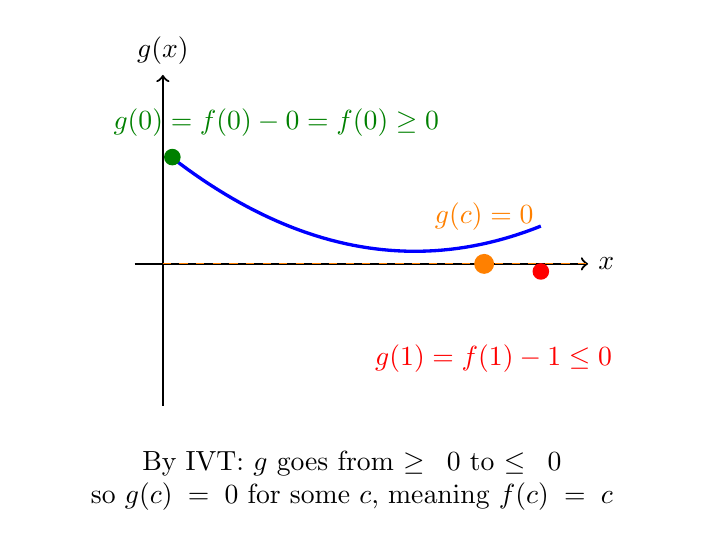
\begin{tikzpicture}[scale=1.2]
    \draw[thick, ->] (-0.3, 0) -- (4.5, 0) node[right] {$x$};
    \draw[thick, ->] (0, -1.5) -- (0, 2) node[above] {$g(x)$};

    % g(x) = f(x) - x
    \draw[blue, very thick, domain=0.1:4, samples=50] plot (\x, {1.2 - 0.8*\x + 0.15*\x*\x});

    % g(0) >= 0
    \fill[green!50!black] (0.1, 1.13) circle (2.5pt);
    \node[green!50!black] at (1.2, 1.5) {$g(0) = f(0) - 0 = f(0) \geq 0$};

    % g(1) <= 0
    \fill[red] (4, -0.08) circle (2.5pt);
    \node[red] at (3.5, -1) {$g(1) = f(1) - 1 \leq 0$};

    % Zero crossing
    \draw[orange, dashed] (0, 0) -- (4.5, 0);
    \fill[orange] (3.4, 0) circle (3pt);
    \node[orange] at (3.4, 0.5) {$g(c) = 0$};

    \node[text width=8cm, align=center] at (2, -2.3) {By IVT: $g$ goes from $\geq 0$ to $\leq 0$\\so $g(c) = 0$ for some $c$, meaning $f(c) = c$};
\end{tikzpicture}
\end{center}

\section{Step by Step}

\begin{center}
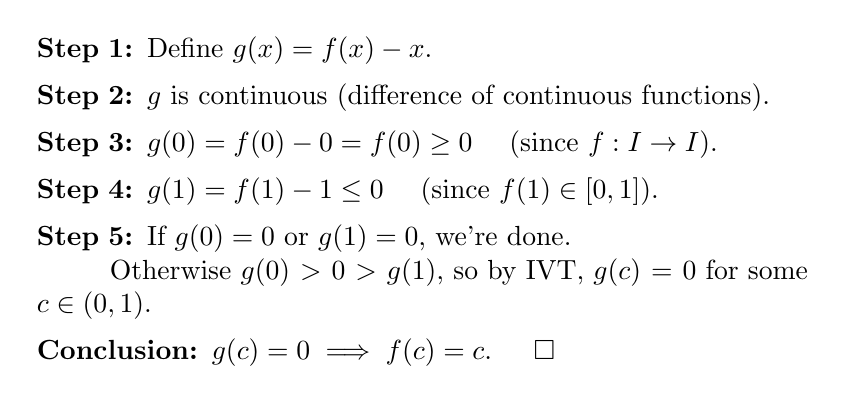
\begin{tikzpicture}[scale=1]
    \node[text width=10cm, align=left] at (0, 0) {
        \textbf{Step 1:} Define $g(x) = f(x) - x$.\\[0.5em]
        \textbf{Step 2:} $g$ is continuous (difference of continuous functions).\\[0.5em]
        \textbf{Step 3:} $g(0) = f(0) - 0 = f(0) \geq 0$ \quad (since $f: I \to I$).\\[0.5em]
        \textbf{Step 4:} $g(1) = f(1) - 1 \leq 0$ \quad (since $f(1) \in [0,1]$).\\[0.5em]
        \textbf{Step 5:} If $g(0) = 0$ or $g(1) = 0$, we're done.\\
        \hspace{2.3em} Otherwise $g(0) > 0 > g(1)$, so by IVT, $g(c) = 0$ for some $c \in (0,1)$.\\[0.5em]
        \textbf{Conclusion:} $g(c) = 0 \implies f(c) = c$. \quad $\square$
    };
\end{tikzpicture}
\end{center}

\section{More Examples}

\begin{center}
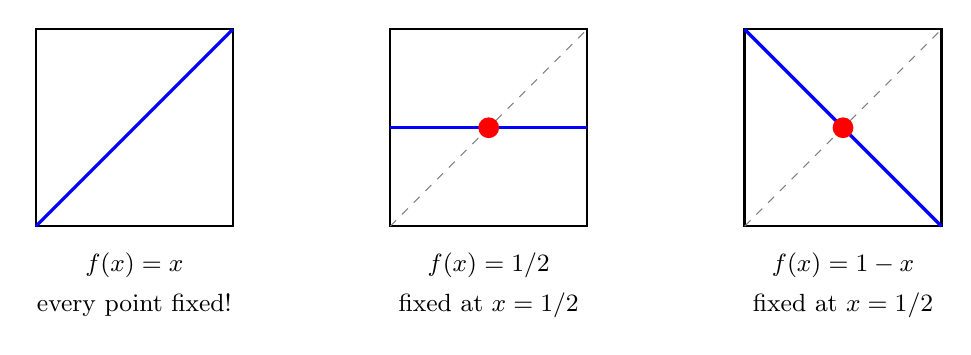
\begin{tikzpicture}[scale=2.5]
    % Example 1: identity
    \begin{scope}[xshift=-1.8cm]
        \draw[thick] (0, 0) rectangle (1, 1);
        \draw[gray, dashed] (0, 0) -- (1, 1);
        \draw[blue, very thick] (0, 0) -- (1, 1);
        \node at (0.5, -0.2) {\small $f(x) = x$};
        \node at (0.5, -0.4) {\small every point fixed!};
    \end{scope}

    % Example 2: constant
    \begin{scope}[xshift=0cm]
        \draw[thick] (0, 0) rectangle (1, 1);
        \draw[gray, dashed] (0, 0) -- (1, 1);
        \draw[blue, very thick] (0, 0.5) -- (1, 0.5);
        \fill[red] (0.5, 0.5) circle (1.5pt);
        \node at (0.5, -0.2) {\small $f(x) = 1/2$};
        \node at (0.5, -0.4) {\small fixed at $x = 1/2$};
    \end{scope}

    % Example 3: 1-x
    \begin{scope}[xshift=1.8cm]
        \draw[thick] (0, 0) rectangle (1, 1);
        \draw[gray, dashed] (0, 0) -- (1, 1);
        \draw[blue, very thick] (0, 1) -- (1, 0);
        \fill[red] (0.5, 0.5) circle (1.5pt);
        \node at (0.5, -0.2) {\small $f(x) = 1-x$};
        \node at (0.5, -0.4) {\small fixed at $x = 1/2$};
    \end{scope}
\end{tikzpicture}
\end{center}

\end{document}
